% Diese Zeile bitte -nicht- aendern.
\documentclass[course=erap]{aspdoc}

%%%%%%%%%%%%%%%%%%%%%%%%%%%%%%%%%
%% TODO: Ersetzen Sie in den folgenden Zeilen die entsprechenden -Texte-
%% mit den richtigen Werten.
\newcommand{\theGroup}{110} % Beispiel: 42
\newcommand{\theNumber}{A212} % Beispiel: A123
\usepackage{amsmath}
\usepackage{graphicx}
\usepackage{caption}
\usepackage{graphicx,subfig}
\usepackage{listings}
\author{Shutao Shen \and Zhiyi Pan \and Yujie Zhang}
\date{Wintersemester 2019/20} % Beispiel: Wintersemester 2019/20
%%%%%%%%%%%%%%%%%%%%%%%%%%%%%%%%%

% Diese Zeile bitte -nicht- aendern.
\title{Gruppe \theGroup{} -- Abgabe zu Aufgabe \theNumber}

\begin{document}
\maketitle

\section{Einleitung}
In dieser Ausarbeitung konzentrieren wir uns auf ein Multicorn-Fraktal, insbesondere das Tricorn-Fraktal. Die Besonderheit des Tricorn-Fraktals ist, dass die Gebilde oder Muster des Tricorn-Fraktals einen hohen Grad von Skaleninvarianz bzw. Selbstähnlichkeit aufweisen.\cite{ wiki:Fraktal} \cite{ wiki:Tricorn} Unsere Aufgabe ist es, ein Tricorn-Fractal zu visualisieren. Dabei müssen 5 vom Benutzer eingegebene Variablen berücksichtigt werden.
\\Wir implementieren unser Projekt hauptsächlich mithilfe von Assembler-Code und von C-Code.


\section{Problemstellung und Spezifikation}
Wir bekommen fünf Parameter vom Benutzer, nämlich \emph{\textbf{r\_start}}, \textbf{\emph{r\_end}}, \textbf{\emph{i\_start}}, \textbf{\emph{i\_end}}, \textbf{\emph{res}} und \textbf{\emph{img}}. Auf der reellen Achse wird durch \emph{\textbf{r\_start}} und \emph{\textbf{r\_end}} und auf der imaginären Achse durch \textbf{\emph{i\_start}} sowie\textbf{\emph{ i\_end}} ein bestimmter Bereich festgelegt. Der Parameter \emph{\textbf{res}} ist die Auflösung(Schrittweite pro Bildpixel) und \textbf{\emph{img}} ist ein Zeiger auf einen Speicherbereich.
\\Um die Aufgabe zu erfüllen, müssen wir alle mögliche \textbf{\emph{ab}}-Kombinationen nach Auflösung und den angegebennen Formeln berechnen, indem wir sie per Interationen mit bestimmter Zahl durchgeführen. Wenn die letzte komplexe Zahl nach \textbf{\emph{n}} mal Iterationen noch beschränkt ist, fäben wir den entsprechende Pixel schwarz, ansonst weiß.
 \begin{equation}
\mathrm{z_{i+1}}=\mathrm{\bar{z}_{i}^{2}}+\mathrm{c}(\mathrm{i} \geq 0) \quad \mathrm{z_{0}}=0
\end{equation}
\begin{equation}\mathrm{c}=\mathrm{a}+\mathrm{bi} \quad \mathrm{a} \in[-2 ; 1] \text { und } \mathrm{b} \in[-1 ; 1]\end{equation}
 Wir berechnen Mächtigkeit vom Wertbereich aus \textbf{\emph{a}} sowie \textbf{\emph{b}} nach den folgenden Formeln. Im folgenden Text nennen wir Mächtigkeit vom Wertbereich aus \textbf{\emph{a}} als Anzahl von \textbf{\emph{a}} analog Anzahl von \textbf{\emph{b}}.
 \begin{equation}
\mathrm{AnzahlVonA}  =\lfloor 3 /\mathrm{res}\rfloor+1   \quad  \mathrm{AnzahlVonB}  =\lfloor 2 / \mathrm{res}\rfloor+ 1
\end{equation}
\textbf{\emph{$a_{i+1}$}} ist Realteil und \textbf{\emph{$b_{i+1}$}} ist Imaginaerteil von \emph{\textbf{$z_{i+1}$}}. Und (\textbf{\emph{$a_{i+1}$}}, \textbf{\emph{$b_{i+1}$}}) ist gemäß der Koordinaten in der komplexen Ebene. Wir berechnen \textbf{\emph{$a_{i+1}$}} und \textbf{\emph{$b_{i+1}$}} durch folgenden Formeln.
\begin{equation}
\label{eq4}
\mathrm{a_{i+1}}= (\mathrm{a_{i}^2}-\mathrm{b_{i}^2})+\mathrm{a}\quad \mathrm{b_{i+1}} = -2*\mathrm{a_{i}}*\mathrm{b_{i}}+\mathrm{b}
\end{equation}
Wir haben bemerkt, dass das Problem des Fließkommaüberlaufs nach einer großen Anzahl von Iterationen auftritt. Deshalb haben wir unsere Formel wie folgt optimiert, um das Problem des Fließkommaüberlaufs bei der Berechung vom Zwischenergebnis nämlich \textbf{\emph{$a^2$}} und \textbf{\emph{$b^2$}} zu vermeiden.
\begin{equation}\mathrm{a_{i+1}}= (\mathrm{a_{i}}-\mathrm{b_{i}}) \cdot (\mathrm{a_{i}}+\mathrm{b_{i}})+\mathrm{a}\end{equation}
Wenn (\textbf{\emph{$a_{i+1}$}},\textbf{\emph{$b_{i+1}$}}) als Koordinaten nach Iteration noch innerhalb der Grenzen des erlaubten Bereichs bleibt, notieren wir dann entsprechend die \textbf{\emph{ab}}-Gruppen.
\\In der obigen Bearbeitung müssen wir die Anzahl der Iterationen dokumentieren sowie wie kann man die entsprechenden \emph{\textbf{ab}}-Gruppen in \textbf{\emph{img}} einspeichern. Zeitgleich sind auch die Probleme des Fließkommaüberlaufs und des Rundungsfehler zu lösen. Dies werden wir in dem nächsten Absatz bearbeiten.


\section{Lösungsansatz}

 \subsection{BMP}
 Um das Fraktal zu visualisieren, müssen wir die Kenntnisse in Bezug auf BMP lernen. BMP ist Abkürzung von Windows Bitmap und bezeichnet ein zweidimensionales Rastergrafikformat.\cite{ wiki:BMP}  Und die Rastergrafiken bestehen aus einer rasterförmigen Anordnung von so genannten Pixeln, denen jeweils eine Farbe zugeordnet ist.\cite{ wiki:Rastergrafik} BMP-Dateien bestehen aus drei Teilen: dem Dateikopf, dem Informationsblock und den Bilddaten. Der Wert bfSize ist im Dateikopf und die Größe der BMP-Datei in Byte.
 \begin{equation}
 \mathrm{bfSize}=54+((\mathrm{biWidth}+\mathrm{AnzahlVonPaddingZero})*3)*\mathrm{biHeight}
 \end{equation}
 54 ist gleich die Größe von Bitmapfileheader plus die Größe von Bitmapinfoheader. Die Bitmapinfoheader-Struktur dient der Beschreibung der Bitmap. Mit den Werten biWidth und biHeight geben wir die Breite bzw. Höhe der Bitmap in Pixeln an.\begin{equation}\mathrm{biWidht}= \mathrm{AnzahlVonA}\end{equation}  \begin{equation} \mathrm{biHeight}= \mathrm{AnzahlVonB}\end{equation}
\\Die Bilddaten werden Zeile für Zeile gespeichert. Wir müssen jede Bildzeile durch rechtsseitiges Auffüllen mit Nullen auf ein ganzzahliges Vielfaches von 4 Bytes ausrichten.
\\Dann schauen wir uns die Bilddaten an. Wir benutzen 24 bpp,\cite{ wiki:BMP} d.h. die Daten jedes Pixels bestehen aus jeweils einem Byte für den Blau-, Grün- und Rot-Kanal. Deshalb drücken  \#ffffff weiß und \#000000 schwarz aus.
 \subsection{Daten speichern}
 In dem C-Code reservieren wir zuerst genügenden Platz für Assembler-Code und dann gilt es die Adresse als Parameter zusammen mit den anderen vier vom Benutzer eingegebenen Parametern an den Assembler-Code weiterzuleiten.
\\In dem Assembler-Code müssen wir jede \textbf{\emph{ab}}-Gruppe beurteilen. Nach dem Vergleich des Iterationsergebnisses mit den obigenannten Kreterien müssen wir eine Konstante \#000000 oder \#ffffff per Bearbeitung in Assembler-Code in die Adresse schreiben. Schließlich soll der Inhalt in der Adresse zuerst per C-Code gelesen werden. Und dann muss der Inhalt für jeder Zeile durch 0 erüllt werden. Und zum Schluss kann ein Bild generiert werden. Und dann schreiben wir die BMP-Datei in die vom Benutzer vorgegebenen Ausgabedatei.
\subsection{Fließkommazahl}
\subsubsection{Rundungsfehler}
Aus der Eigenschaft der Fließkommazahl ergibt sich, dass Fließkommazahl Rundungsfehler enthalten. Um BMP-Datei richtig zu erzeugen, müssen wir sicherstellen, dass jede Zeile die gleiche Anzahl von \textbf{\emph{ab}}-Gruppe aufweist. Deshalb können wir keine While-Schleife verwenden, indem wir jeweils res addieren, um festzustellen, ob die Anzahl der Schleifen den Wertebereich von \emph{\textbf{a}} oder \textbf{\emph{b}} überschreitet. Einerseits ist, dass der Wert von res nach jeder Iteration einen Fehler enthält und die Fehlers sich auch häufen. Und dann kann dies dazu führen, dass die Schleifenanzahl falsch ist. Andererseits ist Ungenauigkeit der Fließkommazahl. D.h. wenn die Zahl sich in der Nähe der Grenze befindet, kann nicht genau bestimmt werden, ob die Zahl größer als die Grenze ist.
\\Stattdessen verwenden wir for-Schleife, um die Anzahl der Schleifen auf der Basis der zuvor kalkulierten Anzahl von \emph{a} und \emph{b} zu bestimmen. Wegen der Existenz von Rundungsfehlern können wir die Anzahl von \emph{a} und \emph{b} nicht unmittelbar durch die obige Formel berechnen, sondern wir müssen $\lfloor x \rfloor$ mit C-Code durch die folgende Formel berechnen
\begin{equation}
\text { Sei } e=\lceil x\rceil- x, x \Leftarrow\left\{\begin{array}{c}{\text {round}(x)+1, \text { wenn } e<0.01} \\ {\lfloor x\rfloor+ 1, \text { sonst }}\end{array}\right.
\end{equation}
und mit Assembler-Code durch die folgende Formel berechnen.
\begin{equation}
\begin{array}{l}{\text { Sei } y=x+0.5} \\ {\quad e=\lceil y\rceil- y, x \Leftarrow\left\{\begin{array}{c}{\text { round }(y+0.5)-1, \text { wenn }|e-0.5|<0.01} \\ {\text { round }(y)-1, \text { sonst }}\end{array}\right.}\end{array}
\end{equation}
\subsubsection{Besonderer Wert}
Bei der Berechnung sind einige spezielle Werte entstanden, die nicht direkt durch normalen Vergleich beurteilt werden können, ob sie größer als die Grenze sind, hier wie z.B. INF und NAN. Deshalb müssen wir uns mit diesen speziellen Werten separat auseinandersetzen.
\\Wir bestimmen eine Fließkommazahl direkt durch ucomiss, ob sie NaN(Not a Number) ist. Anschließend wird der absolute Wert dieser Zahl genommen und mit \emph{FLT\_MAX} verglichen, um zu bestimmen, ob die Zahl inf ist, denn Inf(Infinity) ist größer als alle Zahlen.
\subsection{Anzahl der Iterationen}\label{Anzahl_der_Iterationen}
Um die Anzahl von Iterationen am besten zu entscheiden, haben wir einen Test in der Programmiersprache C geschrieben, indem wir so viel Situationen wie möglich laufen und eine mindestens benötigende Iterationsanzahl zusammenfassen. Denn nach Eigenschaft der Mandelbrot-Menge wissen wir: für alle c gehört zu Mandelbrot-Menge, soll $|z_n| \leq 2$, legen wir die erste vier Parameter in Funktion 'multicorn' fest, Wir nehmen hierbei noch an, dass die Auflösung mit 0.001 an fängt. Wir erhöhen die Anzahl der Iterationen kontinuierlich und gleichzeitig bilden wir das Bild aus jeder Ausführung mit dieser neusten Zahl als Eingabe. Dieses Bild vergleichen wir mit dem bei 500 Iterationen gebildeten Bild. Sobald beide Bilder eine mehr als 99.9\%ige Ähnlichkeit aufweisen, notieren wir die momentane Iterationsanzahl un prüfen wir die nächsten fünf Bilder aus den weiteren Iterationen. Wenn alle fünf die Bedingung erüllen können, halten wir diese Anzahl von Iterationen für die beste Anzahl von Iterationen. Nachdem wir eine gasamte Statistik aller Auflösungen, die im Intervall [0.001;1] mit einem Abstand von 0.001 zu erstellen sind, auf die gleiche Weise getestet haben, haben wir folgenden Daten bekommen.
\begin{lstlisting}
Arguments:
r_start:-2.000000, r_end:2.000000, i_start:-2.000000, i_end:2.000000
res: from 0.001000 to 1, step:0.001000, total:1000
	res:0.001000 => min_Iteration_num:219
	res:0.002000 => min_Iteration_num:216
	res:0.003000 => min_Iteration_num:220
            .............
	res:0.998000 => min_Iteration_num:5
	res:0.999000 => min_Iteration_num:6
	res:1.000000 => min_Iteration_num:2
\end{lstlisting}
Um eine angemessene Iterationsanzahl für allgemeine Situation davon zu finden, benutzen wir die Funktion TRIMMEAN(array, 0.1) von Excel. TRIMMEAN schließt zuerst 5\% Werte vom oberen und 5\% von unteren Rand des Datensatzes aus und berechnet dann den Durchschnitt. Das Ergebnis ist 69.1544. Und bei anderen Testen mit verschiedenen Grenzen und Auflösung ist es analog. Deshalb benutzen wir danach 70 als die Anzahl von Iterationen.
\section{Dokumentation der Implementierung}
\subsection{Benutzer-Dokumentation}
\begin{itemize}
\item[*]\textbf{\emph{USAGE:tricorn [options]}}
\item[*]\textbf{\emph{-a, --r\_start  float}}
\\-Legen Sie einen Gleitkommawert als Untergrenze der reellen Zahl fest. Er sollte nicht grösser als \emph{\textbf{r\_end}} sein.
\item[*]\textbf{\emph{-b, --r\_end float}}
\\-Geben Sie einen Gleitkommawert als Obergrenze der reellen Zahl ein. Er sollte nicht kleiner als \emph{\textbf{r\_start}} sein.
\item[*]\textbf{\emph{-c, --i\_start  float}}
\\-Setzen Sie einen Gleitkommawert als Untergrenze der imaginären Zahl. Er sollte nicht grösser als \emph{\textbf{i\_end}} sein.
\item[*]\textbf{\emph{-d, --i\_end  float}}
\\-Setzen Sie einen Gleitkommawert als Obergrenze der imaginären Zahl. Er sollte nicht kleiner als \emph{\textbf{i\_start}} sein.
\item[*]\textbf{\emph{-r, --res  float}}
\\-Legen Sie einen Gleitkommawert als Auflösung für Pixel fest
\item[*]\textbf{\emph{-o, --output  location}}
\\- Geben Sie eine Adresse ein, die genügend Speicherplätze haben muss.
\item[*]\textbf{\emph{-h, --help}}
\\-Diese Nachricht drucken und beenden
\end{itemize}
Der empfohlene Wertebereich von \textbf{\emph{r\_start}}, \textbf{\emph{r\_end}}, \textbf{\emph{i\_start}}, \textbf{\emph{i\_end}}, mit dem man das ganze Bild bekommen kann, lautet $[2,float\_max]$. Und \textbf{\emph{res}} muss größer als 0 sein, am besten größer als 0,00001 sein. Denn wenn res zu klein ist, ist die BMP-Datei zu groß. Das Programm überprüft nicht nur Anzahl von Parametern, sondern auch die Korrektheit der Eingaben. Wenn ungültige Parameter eingegeben werden, meldet das Programm Fehler, z.B. wenn man nur \emph{\textbf{r\_start}} eingibt, gibt Programm wie folgend aus:
\begin{lstlisting}
r_end - wrong or not given
usage: ./tricorn [options]
options:
-a, --r_start   [float] -the value as lower bound of real number.
-b, --r_end     [float] -the value as upper bound of real number.
-c, --i_start   [float] -the value as lower bound of imaginary number.
-d, --i_end     [float] -the value as upper bound of imaginary number.
-r, --res       [float] -the value as resolution of the picture.
-o, --output    [string]-the path of the output image file.
-h, --help              -print the help message.
example:
tricorn --r_start -2 --r_end 2 --i_start -2 --i_end 2 --res 0.01 --output './output.bmp'
\end{lstlisting}
\subsection{Makefile}
Zur Anwendung von Makefile gibt es 16 Befehle: \textbf{\emph{all}}, \textbf{\emph{example}}, \textbf{\emph{testIterationNum}}, \textbf{\emph{testCorrection}}, \textbf{\emph{testPerformance}}, \textbf{\emph{build}}, \textbf{\emph{clean}}, \textbf{\emph{runMain}}, \textbf{\emph{runMainExample}}, \textbf{\emph{buildWithCImp}}, \textbf{\emph{buildTestIterationNum}}, \textbf{\emph{runTestIterationNum}}, \textbf{\emph{buildTestCorrection}}, \textbf{\emph{runTestCorrection}}, \textbf{\emph{buildTestPerformance}}, \textbf{\emph{runTestPerformance}}. Die ersten 5 dabei sind abhängig von anderen übrigen und werden öfter benutzt, deshalb wird hier diesen Teil mehr fokussiert.
\begin{itemize}
\item[*]\textbf{\emph{all: build runMain}}
\\-Die Hauptdatei von Compiler generieren und dann ausführen.
\item[*]\emph{\textbf{example: build runMainExample }}
\\-Die Hauptdatei von Compiler generieren und dann mit vordefinierte Eingaben ausführen.
\item[*]\textbf{\emph{testIterationNum: buildTestIterationNum runTestIterationNum}}
\\–Datei,die die rationale Nummer für Iteration in Hauptprogram testet, von Compiler generieren und dann ausführen.
\item[*]\emph{\textbf{testCorrection: buildTestCorrection runTestCorrection }}
\\–Datei, die die Korrektheit dieses Programs per Vergleich mit dem Standardscode testet, von Compiler generieren und dann ausführen.
\item[*]\textbf{\emph{testPerformance: buildTestPerformance runTestPerformance }}
\\– Datei,die die Performance dieses Programs per Vergleich mit dem Standardscode testet, von Compiler generieren und dann ausführen.	
\item[*]\emph{\textbf{clean}}
\\-Löschen alle frühzeitige Operationen.
\item[*]\textbf{\emph{buildWithCImp}}
\\-Kompilieren und führen das ganzen Projekt mit einer C-Datei als Ersetzung des Assemble-Anteils aus.
\end{itemize}
\subsection{Entwickler-Dokumentation}
Es gibt insgesamt 4 Programme, nämlich test\_performance.c, test\_correction.c, iteration\_number.c und tricorn.c. 
\subsubsection{Hauptprogram}
Das ganze Program bestehen aus 2 Daten, nämlich tricorn.c und multicorn.S. Das c-Datei bekommt die Argumente vom Benutzer und prüfen die korrektheit. Wenn alle Argumente richtig sind, läuft das Program wie folgt: \newline
C-Program reserviert den passenden Speicherplatz für img, gibt den Zeiger zusammen mit von Benutzer bekommende Argumente dem Assembler-Program ein. Das Assembler-Datei bearbeitet die pixels Zeile für Zeile mit SIMD Instructions, d.h. jedes mal 4 Daten mit dem Formel (\ref{eq4}) berechnen, Dummy-datei wird gefüllt, wenn die Anzahl von Daten weniger als 4. Nach der berechnung, die Gültigkeit von den Daten wird zuerst geprüft, danach die Grenze.
\subsubsection{Test-program}
Das Test-program bestehen aus 3 Teile: testIterationNum, testCorrection, testPerformance.\newline
testIterationNum: Das ganze Program bestehen aus 2 Daten, nämlich iteration\_number.c und multicorn\_c\_test\_double\_with\_step.c. Die Hauptidee ist gleich wie  (\ref{Anzahl_der_Iterationen}). Die multicorn Function hier wird geändert, es kann Schritt für Schritt rechnen, um die Geschwindigkeit zu verbessern. \newline
testCorrection: Das ganze Program bestehen aus 3 Daten, nämlich test\_correction.c, multicorn\_c\_test\_double.c und multicorn.S. Die Hauptidee ist gleich wie  (\ref{correction}). Die visualisierung von den Fehler wird im Ordner correction sichern.\newline
testPerformance: Das ganze Program bestehen aus 3 Daten, nämlich test\_performance.c, multicorn\_c\_test\_double.c und multicorn.S. Die Hauptidee ist gleich wie  (\ref{performance}).
% TODO: Je nach Aufgabenstellung einen der Begriffe wählen
\section{Genauigkeit}\label{correction}
Wir müssen jetzt die Genauigkeit testen.
Zuerst erzeugen wir Standardbild durch C-Code und der Gedankengang ist wie folgende Pseudocode.
\begin{lstlisting}[mathescape=true]
For each pixel ($a_0$, $b_0$), do:
{
    init($a$, $b$);
    Loop n times:
        ($a$, $b$) <= ( $a^2$ + $b^2$ + $a_0$, $-2*a*b$ + $b_0$);
    check_print($a_0$, $b_0$, $a$, $b$);
}
\end{lstlisting}
Die Genauigkeitsrate entspricht der Anzahl der Pixels, die gleich wie was in Standardbild ist, durch die Anzahl aller Pixel in einen Foto, was durch unseren Program dagestellt ist. Damit die genauer sein kann, berechnen wir einen Durchschnitt zahlreicher Genauigkeiten aus verschiedenen Aufrufen. Die Strategie ist so: wir beginnen mit \textbf{\emph{r\_start}} = -2, \emph{\textbf{r\_end}} = 2, \textbf{\emph{i\_start}} = -2, \emph{\textbf{i\_end}} = 2. Jedes Mal setzen wir \textbf{\emph{r\_start}} = \emph{\textbf{r\_start}} * 2, \textbf{\emph{r\_end}} = \emph{\textbf{r\_end}} * 2, \textbf{\emph{i\_start}} = \textbf{\textbf{i\_start}} * 2, \emph{\textbf{i\_end}} = \textbf{\emph{i\_end}} * 2, bis \emph{\textbf{r\_start}} und \textbf{\emph{i\_start}} gleich $-2^{99}$ und \emph{\textbf{r\_end}} und \textbf{\emph{i\_end}} gleich $2^{99}$ sind. Wir müssen Randfall testen. Deshalb testen wir auch den Fall, wenn \emph{\textbf{r\_start}} und \textbf{\emph{i\_start}} gleich \emph{FLT\_MAX} und \emph{\textbf{r\_end}} und \textbf{\emph{i\_end}} gleich \emph{FLT\_MAX} sind. Für jede Kombination von Grenzwerten testen wir \emph{\textbf{res}} separat. \textbf{\emph{res}} ist von 0,001 bis 1 und werden jedes Mal um 0,001 erhöht. Dann zeichnen wir die Genauigkeitsrate dazu auf. Schließlich berechnen wir die durchschnittliche Genauigkeitsrate, die dem Grenzwert entspricht.
\begin{lstlisting}
Arguments:
r_start:-2, r_end:2, i_start:-2, i_end:2
res: from 0.001000 to 1, step:0.001000, total:1000
	res:0.001000 => accuracy:0.998964, diff_pixels:6221
	res:0.002000 => accuracy:0.999304, diff_pixels:1045
                  ....................
    res:1.000000 => accuracy:0.916667, diff_pixels:1
summary: 966/1000 test, 96.600% perfect match,average_accuracy:99.985%
\end{lstlisting}
Dann berechnen wir die durchschnittliche Genauigkeit basierend auf der gesamten Genauigkeit. Zum Schluss beträgt die endgültige Genauigkeit unseres Programms 99,998\%.
 \begin{lstlisting}[mathescape=true]
r_start:$-2^2$, r_end:$2^2$, i_start:$-2^2$, i_end:$2^2$
res: from 0.001000 to 1, step:0.001000, total:1000
summary: 968/1000 test, 96.800% perfect match, average_accuracy:99.997%
                       ....................
r_start:-FLT_MAX, r_end:FLT_MAX,i_start:-FLT_MAX,i_end:FLT_MAX,
res: from 0.001000 to 1, step:0.001000, total:1000
summary: 964/1000 test, 96.400% perfect match, average_accuracy:99.997%

total_summary: total_average_accuracy:99.998%
\end{lstlisting}
Das folgende Bild ist ein Beispiel über Korrektheit mit der bestimmte Grenze. Wir zeigen nur fehlerhafte Daten im folgenden Diagramm.
\begin{figure}[htb]
\centering
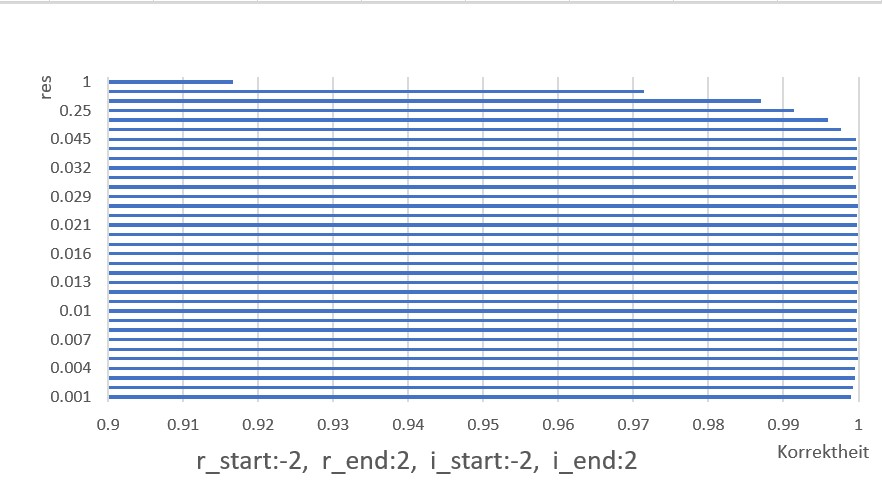
\includegraphics [width=7cm] {Korrektheit.jpg}
\caption{r\_start=-10,r\_rnd=10,i\_start=-10,i\_end=10}
\label{fig:label}
\end{figure}
\\Zum Beispiel wenn der Benutzer die folgenden Parameter eingibt, zeigt unser Programm das folgende Bild.
\begin{figure}[htb]
\centering

\includegraphics [width=7cm] {ddd.png}
\caption{r\_start=-10,r\_rnd=10,i\_start=-10,i\_end=10,res=0.001}
\label{fig:label}
\end{figure}
\\Wir wählen ein exponentielles Wachstum für den Grenzwert anstelle eines linearen Wachstums. Der Grund dafür ist, dass Benutzer eher kleinere Zahlen eingeben. Wir müssen am Anfang mehr Grenzwerte testen. Bei großen Zahlen ist die Wahrscheinlichkeit einer Benutzereingabe nicht hoch. Wir dürfen weniger Grenzwerte testen. Dies verbessert die Effizienz bei garantierter Genauigkeit.

Unser Programm kann keine 100\%ige Genauigkeit erreichen. Es wird einige ungenaue Daten geben. Diese Daten können visualisiert werden. Wie in dem folgenden Bild gezeigt, ist der rote Punkt die Fehlerstelle. Wir glauben jedoch, dass diese Fehler in einem vernachlässigbaren Bereich liegen.
\begin{figure}[htb]
\centering
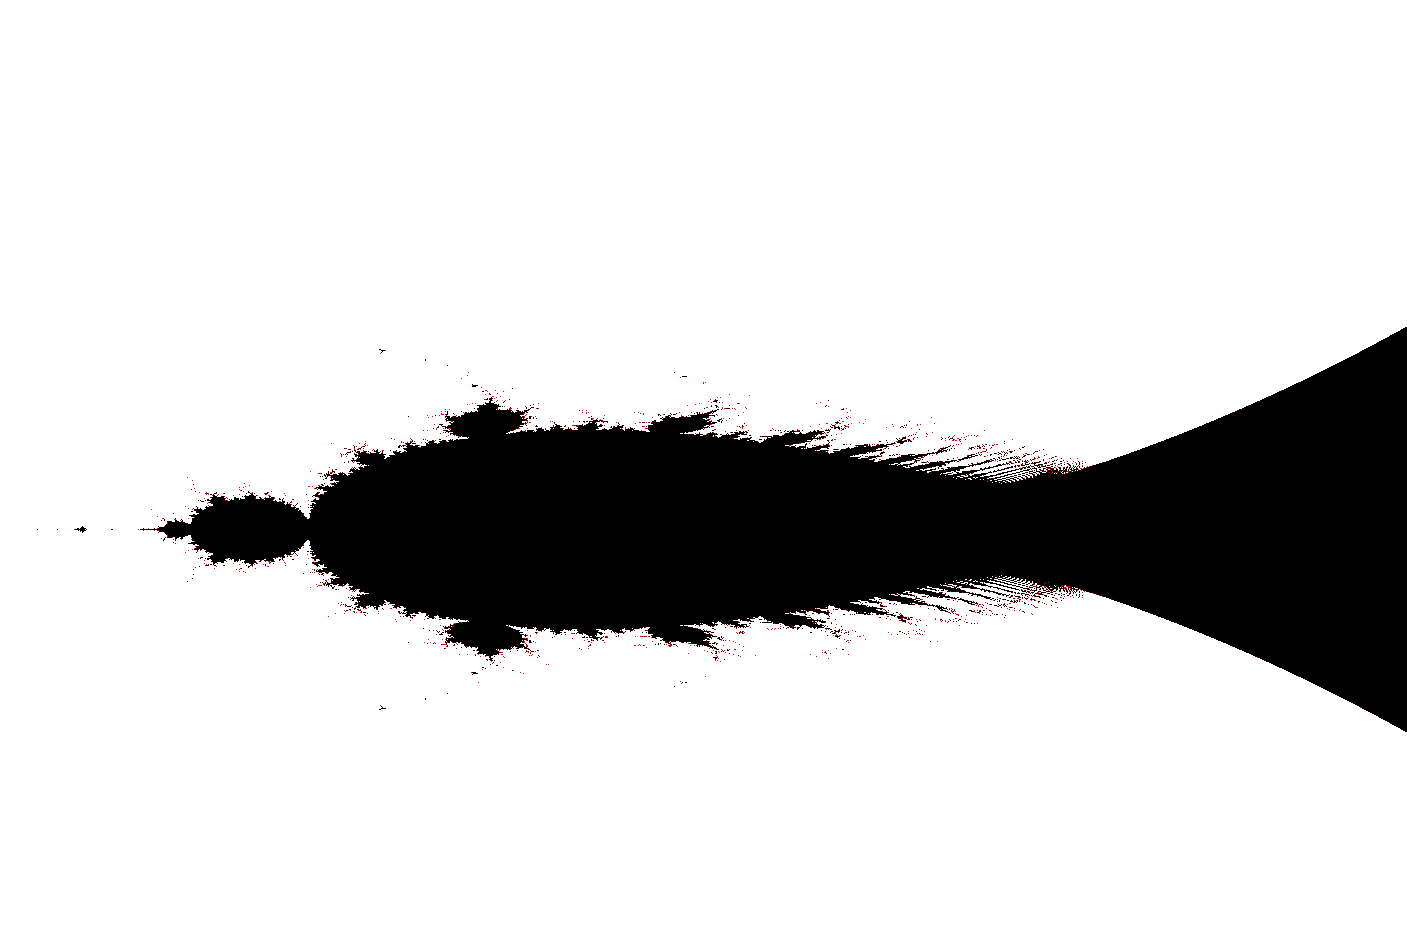
\includegraphics[width=10cm]{Genauigkeit.png}
\caption{Genauigkeit}
\label{fig:label}
\end{figure}


\section{Performanzanalyse}\label{performance}
\subsection{Performanz}
Wir setzen eine Regel: \emph{\textbf{res}} erhöht sich von 0,001 auf 1 und jedes Mal um 0,001. Wir berechnen: Die Laufzeit der Program in Assembler und die Laufzeit der entprechenden Program in C. Wir können die folgenden Daten erhalten.
 \begin{lstlisting}
 r_start:-2.000000, r_end:2.000000, i_start:-2.000000, i_end:2.000000
res: from 0.001000 to 1, step:0.001000, total:1000
	res:0.001000
		assembly_code: 	run_time:0.343072 s
		c_code: 	run_time:0.993629 s
	res:0.002000
		assembly_code: 	run_time:0.076925 s
		c_code: 	run_time:0.248449 s
                ..............
    res:0.999000
		assembly_code: 	run_time:0.000001 s
		c_code: 	run_time:0.000002 s
	res:1.000000
		assembly_code: 	run_time:0.000001 s
		c_code: 	run_time:0.000002 s
\end{lstlisting}
Um deutlicher zu sehen,haben wir auch fogenden Diagramm erstellt.
\begin{figure}[htb]
\centering
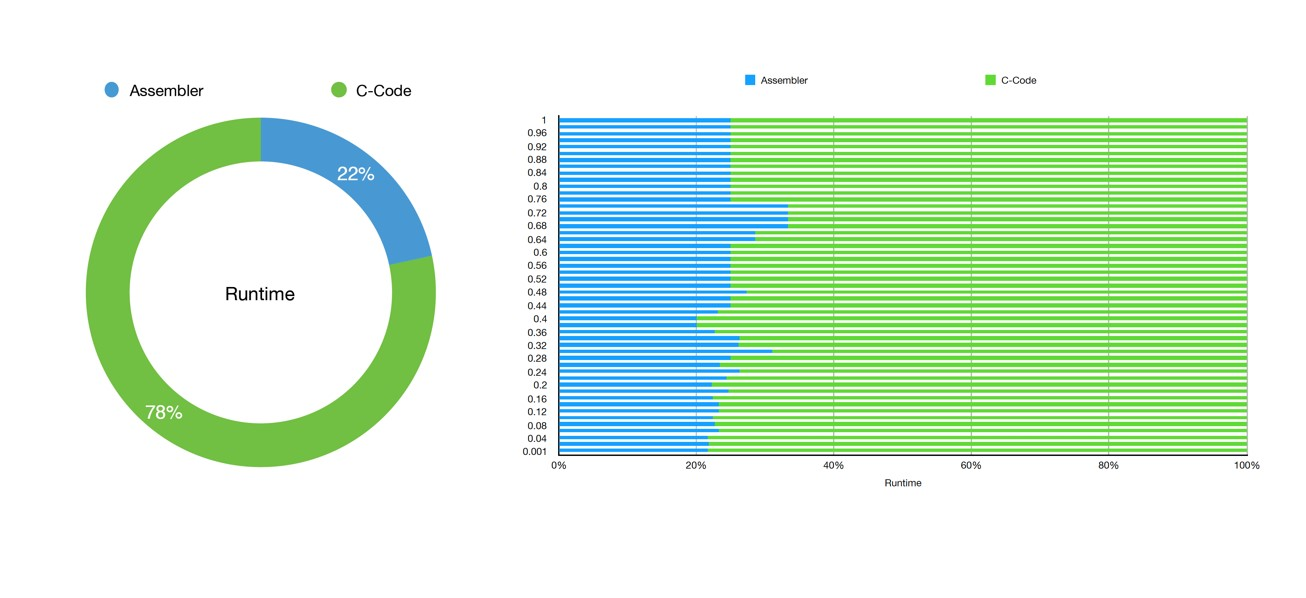
\includegraphics[width=10cm]{Runtime.jpg}
\caption{Runtime}
\label{fig:label}
\end{figure}

Durch dieses Diagramm über Laufzeit kann man klar entdecken, dass der Assembler  schneller laufen kann. Grund dafür kann man in diene Teil deutlich zeigen:
Die folgende beide Code berechnen $\mathrm{a^2} -\mathrm{b^2}$. Eine ist Assembler-Code und die andere ist Disassembly-Code.
 \begin{lstlisting}
//Assembler-Code
subps  xmm10, xmm14
addps  xmm14, xmm13
mulps  xmm10, xmm14

//Disassembly-Code
addss  xmm1, DWORD PTR [rbp-0x34]
movss  xmm0, DWORD PTR [rbp-0x38]
subss  xmm0, DWORD PTR [rbp-0x34]
mulss  xmm0, xmm1
 \end{lstlisting}
Im Vergleich zu Disassembly-Code können wir feststellen, dass c während Iteration einmal jeweils nur eine Fleißkommazahl verarbeitet. In unserem Programm verwenden wir während Iteration so viel wie möglich die SIMD-Einheit, um 4 Fließkommazahlen paralle zu verarbeiten.
\\Geschwindigkeit hängt von zwei Faktoren ab. Eine ist, je größer die Anzahl der Iterationen ist, desto größer ist die Differenz zwischen der Geschwindigkeit von Assembler und der Geschwindigkeit von c. Andere ist, wenn $\mathrm{AnzahlVonA}$ modulo 4 gleich 0 ist, ist schnellste Geschwindigkeit. Wenn \{$\mathrm{AnzahlVonA} \bmod 4 \neq 0$\}, je größer das Ergebnis von \{$\mathrm{AnzahlVonA} \bmod 4$\} ist, desto schneller ist die Geschwindigkeit. Das ist Randeffekt.

\subsection{Weitere Optimierung}
Um unser Programm zu optimieren, studieren wir die Grundeigenschaft von Tricorn-Fraktalen. Wir haben eine sehr nützliche Eigenschaft von Tricorn-Fraktalen gefunden, nämlich dass die \textbf{\emph{ab}}-Gruppe die Bedingung erfüllt: gdw. $\sqrt{a^{2}+b^{2}}$ kleiner als 2.\cite{wiki:mandelbrot}Es gibt einen kleinen Unterschied zwischen unsere und die Formel von Wikipedia. Unsere Formel ist $\mathrm{z_{i+1}}=\mathrm{\bar{z}_{i}^{2}}+\mathrm{c}(\mathrm{i} \geq 0)$. Die Formel von Wikipedia  ist $\mathrm{z_{i+1}}=\mathrm{{z}_{i}^{2}}+\mathrm{c}(\mathrm{i} \geq 0)$. Aber wir können beweisen, dass die Eigenschaft für unsere Formel auch gilt. Mathematische Probleme zu lösen ist nicht das Hauptgewicht unserer Aufgabe. Deshalb werden wir sie hier nicht erläutern.
\\Um diese Formel zu benutzen müssen wir nicht alle möglichen \emph{\textbf{ab}}-Kombinationen überprüfen, sondern nur die, die diese Voraussetzung erfüllen. Diese Formel verbessert die Laufgeschwindigkeit theoretisch erheblich.

\section{Zusammenfassung und Ausblick}
Schließlich haben wir das Problem der Bilderzeugung von Tricorn-Fraktalen erfolgreich gelöst. In dem Prozess haben wir unsere Kenntnisse über Fließkommazahlen bzw. Bitmap-Dateien erweitert. Wir haben die Programmoptimierung abgeschlossen und liefern auch Ideen für die mathematische Optimierung. Wir haben auch bemerkt, dass die Leistung von Assembler besser als C-Code ist.
\\Bis zu diesem Zeitpunkt ist unser Projekt beendet. Wir sind auf viele Schwierigkeiten gestoßen, doch haben wir die überwunden. Wir sind ganz spannend und zufrieden mit unsereren Ergebnissen.


% TODO: Fuegen Sie Ihre Quellen der Datei Ausarbeitung.bib hinzu
% Referenzieren Sie diese dann mit \cite{}.
% Beispiel: CR2 ist ein Register der x86-Architektur~\cite{intel2017man}.
\bibliographystyle{plain}
\bibliography{Ausarbeitung}{}



\end{document}